\chapter{Imitation Learning}
Imitation learning is also called behavioral cloning. The basic idea of imitation learning is ``train to fit the expert behavior''. In other words, given a demonstration, we want to make the agent follow the demonstration as closely as possible, to best imitate the demonstration's behaviors.
\section{Distribution Mismatch}
However, a big problem of such type of approach is that it does not generalize well, if at all. For example, one can imagine that the agent makes a small mistake and ends up being in a slightly different state that what it has seen (trained) before, but since the state is novel, the agent does not know how to act, thus behaving randomly, diverging from the learned trajectory. An illustration of such mismatches is shown in Fig. \ref{fig:imitation_div}.
\begin{figure}
    \centering
    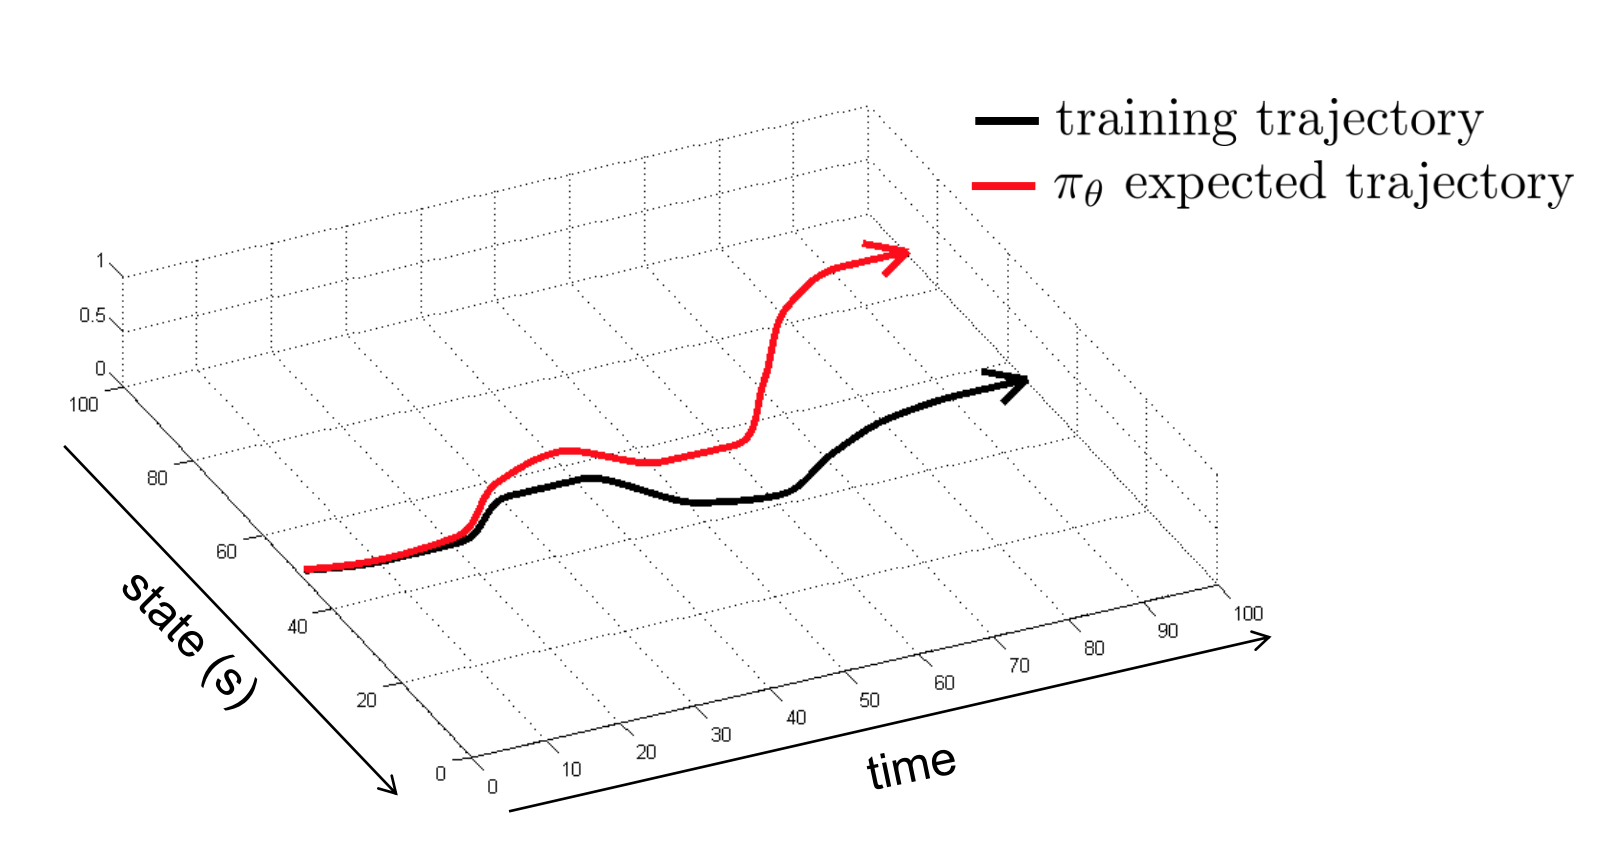
\includegraphics[scale = 0.3]{figures/imitation_div.png}
    \caption{Mistakes aggregate in behavior cloning.}
    \label{fig:imitation_div}
\end{figure}
\section{Dataset Aggregation}
The aggregation of mistakes that the agent makes often makes imitation learning not feasible. But imitation learning does work in some cases. Intuitively, if the agent could somehow learn from the mistakes, and we keep appending data to the agent's dataset so that the agent is exposed to a variety of states. If the actions applied to those states are correct, then eventually, the agent can, ideally, converge to an optimal trajectory. This is essentially the idea behind an imitation learning algorithm called Dataset Aggregation (DAgger) \cite{ross2011reduction}.
\begin{algorithm}[t!]
\caption{Dataset Aggregation (DAgger)}
\begin{algorithmic}[1]
\label{alg:dagger}
\REQUIRE Human data $\mathcal{D} = \{o_1,a_1,...,o_N,a_N\}$

\WHILE{true}
    \STATE Train $\pi_\theta(a_t|o_t)$ from human data $\mathcal{D} = \{o_1,a_1,...,o_N,a_N\}$.
    \STATE Run $\pi_\theta(a_t|o_t)$ to get dataset $\mathcal{D}_\pi = \{o_1,...,\o_M\}$
    \STATE Ask human to label $\mathcal{D}_\pi$ with actions $a_t$
    \STATE Aggregate $\mathcal{D} \leftarrow \mathcal{D} \cup \mathcal{D_\pi}$
\ENDWHILE
\RETURN optimal imitation-learned trajectory as $\tau^{return}$
\end{algorithmic}
\end{algorithm}
In step 3 of Algorithm \ref{alg:dagger}, what we are doing is basically discarding the actions from running trained policy $\pi_\theta(a_t|o_t)$. Instead, we ask a human in the loop to label what they would have done based on the observations in $D_\pi$. Take an autonomous car for example, the training data would be images labeled with steering commands, and we let the car collect more data, which are only images. Then we give those images to a human, and let the human determine, based on each image, what action (steer left, right, or go straight) that the human would have applied if he observed such an image.

It can be proven that DAgger resolves the distribution ``drift'' issue. However, one problem with DAgger is that human might be error-prone, so the human labelled data might be flawed to use. Furthermore, more subtly, human, in most cases, does not make decisions based on a Markovian process. Therefore, the current time step's action might be dependent on a state/observation some number of time steps ago.
\section{When Does Imitation Learning Fail?}
In general, there are some cases where one may fail to fit the expert data, which lead to undesirable outcomes of imitation learning.
\subsection{Non-Markovian Behaviors}
First, the data is Non-Markovian, as mentioned above. Actually Non-Markovian process is more natural and intuitive for human in that human learns from their past mistakes. Why is this wrong? Essentially, we are fitting the wrong distribution. Since we are fitting a policy distribution based on a Markovian process, our goal is fitting $\pi(a_t|o_t)$. However, if the expert data is not Markovian, then we are trying to fit $\pi(a_t|o_t)$ from another distribution $\pi(a_t|o+1,...,o_t)$. One solution is to use a lot of previous memory frames, and concatenate them as one huge frame, effectively augmenting the state space. However, this solution might generate too many weights, increasing the computation complexity. Another solution is that one can fit the expert data using an RNN with shared weights, and one possible implementation is shown in Fig. \ref{fig:im_RNN}.
\begin{figure}
    \centering
    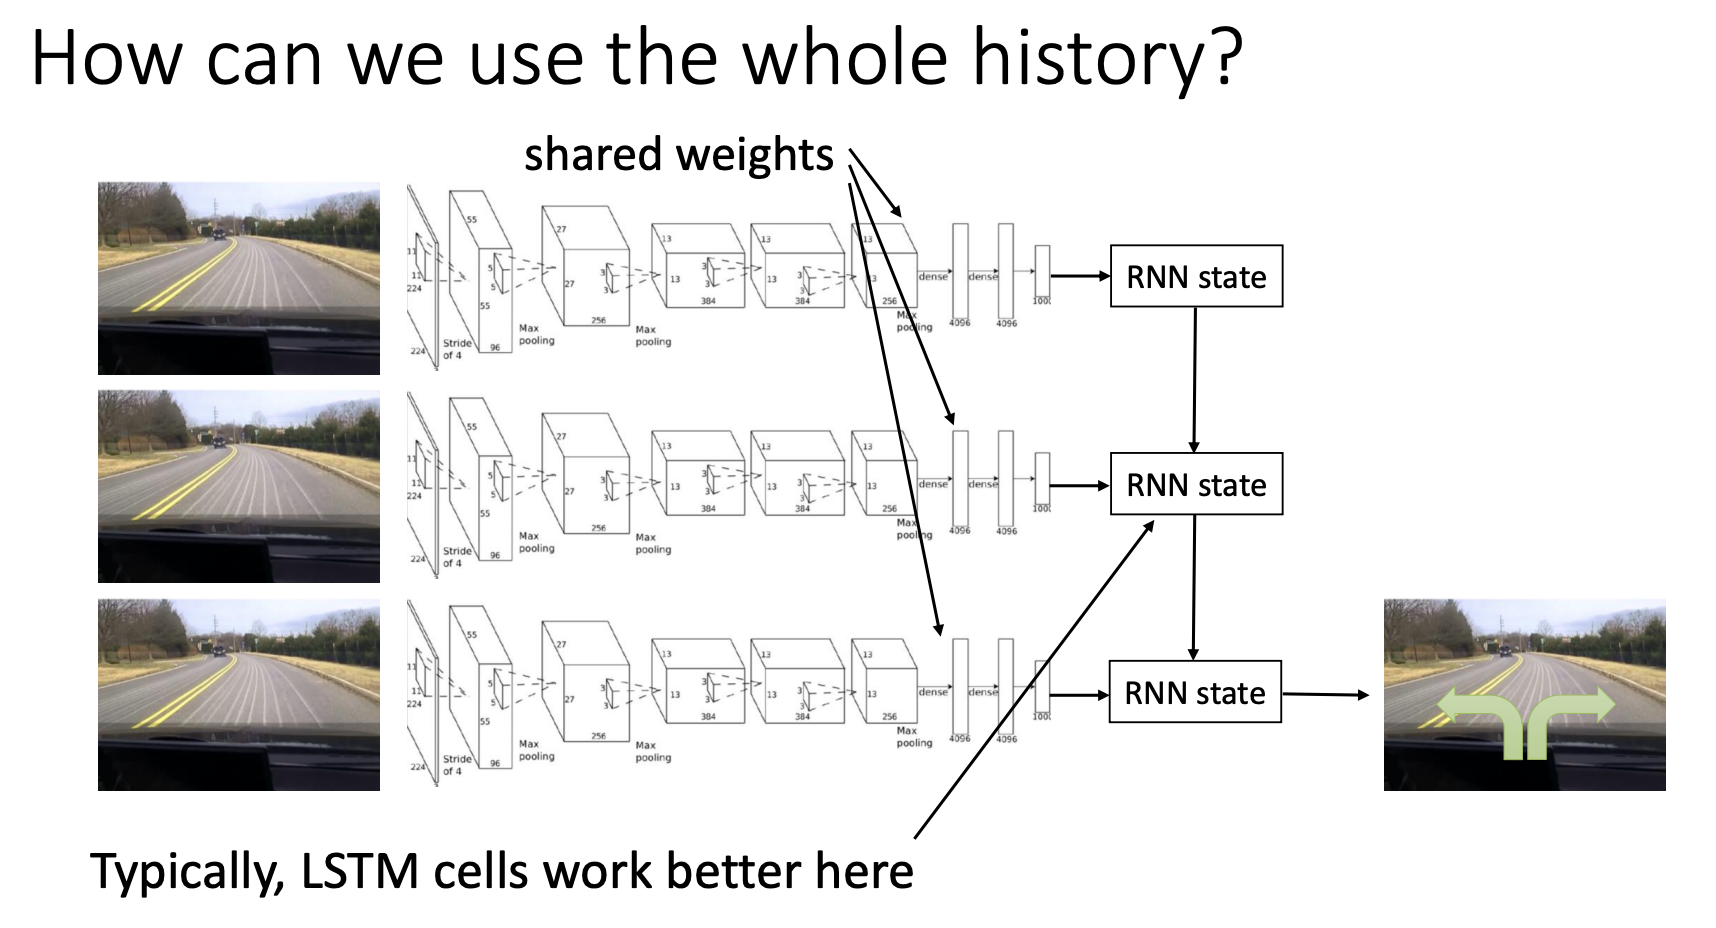
\includegraphics[scale = 0.4]{figures/im_RNN.png}
    \caption{Using RNN to address non-Markovian expert data.}
    \label{fig:im_RNN}
\end{figure}
The underlying reason why having a full history makes imitation learning difficult is that history data tends to exacerbate the causality misclassification. Having more history might make the agent learn the wrong direction of causality, and in many cases, the wrong direction is actually easier to learn. For more information, please refer to this paper \cite{de2019causal}.
\subsection{Multimodal Behaviors}
Another scenario where fitting expert might fail is that the expert has \textbf{multimodal} behaviors. An example of this is that when you are controlling a drone to dodge a tree ahead, you either steer left or steer right. However, if you choose the wrong parametric form of the distribution (e.g. a simple Gaussian) of the actions, the distribution might average out left and right and choose to go straight, as shown in figure \ref{fig:multimodal}.
\begin{figure}
    \centering
    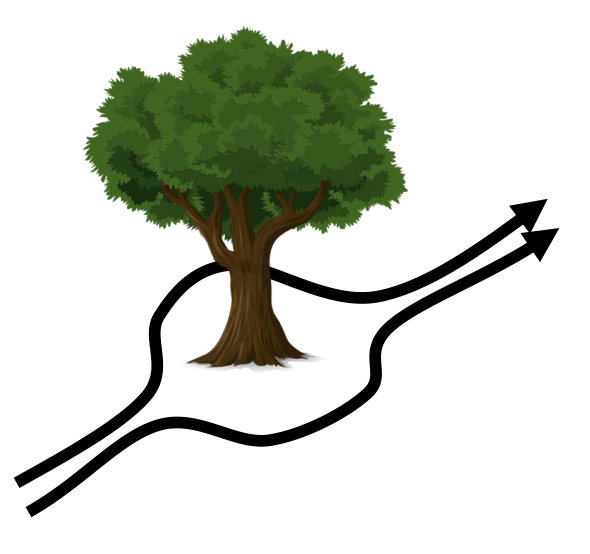
\includegraphics[scale=0.5]{figures/multimodal.png}
    \caption{Multimodal behaviors.}
    \label{fig:multimodal}
\end{figure}
Some methods to mitigate this issue include: first, one can use a mixture of different Gaussian distributions, instead of just one. Second, construct a latent space variables model, which we will talk more about in variational inference. Third, we can use autogregressive discretization. Specifically, a mixture of Gaussians means that the policy distribution should be a weighted sum of different Gaussians with different means and variances. 
\section{Theoretical Analysis of Imitation Learning's Error}
First we define two different reward functions for imitation learning. To make our analysis easier, we assume the policy function is deterministic. First, we can define the reward function as $r(s,a)=\log p(a=\pi^*(s)|s)$. This function measures the log likelihood of the action equal to expert policy's action. Another (simpler) choice can just be a counter to count the number of mistakes. Specifically, 
\[ c(s,a) = \begin{cases} 
          0 & \text{if } a = \pi^*(s) \\
          1 & \text{o.w.}
       \end{cases}
    \]
To analyze this, let's introduce a lower bound on the probability of making mistakes: $\pi_\theta(a\neq \pi^*(s)|s)\leq \epsilon$ for all $s\sim p_{train}(s)$. The fit distribution of states $p_\theta(s)$ is consisted of two parts: the first part is the probability of no mistakes made, and the second part is the probability of making some mistakes. Using Baye's rule, we can calculate $p_\theta(s)$ as follows:
$$p_\theta(s_t) = (1-\epsilon)^tp_{train}(s_t)+(1-(1-\epsilon)^t)p_{mistake}(s_t)$$
so to measure the divergence of $p_\theta$ from $p_{train}$, we take the difference of the two distriutions (naive):
$$|p_\theta(s_t)-p_{train}(s_t)|=(1-(1-\epsilon)^t)|p_{mistake}-p_{train}|\leq2(1-(1-\epsilon)^t)$$
$$\leq 2\epsilon t$$
where we used the identity that $(1-\epsilon)^t\geq1-\epsilon t$ for $\epsilon\in [0,1]$. Thus, we can calculate the expected number of mistakes the agent makes using this scheme by:
$$\sum_t\mathbb{E}_{p_\theta(s_t)}[c_t] = \sum_t\sum_{s_t}p_\theta(s_t)c_t(s_t)\leq\sum_t\sum_{s_t}p_{train}(s_t)c_t(s_t)+|p_\theta(s_t)-p_{train}(s_t)|c_{max}$$
$$\leq\sum_t\epsilon+2\epsilon t$$
$$\in O(\epsilon T^2)$$
Also note that with DAgger $p_{train}(s)\rightarrow p_\theta(s)$. So we no longer have the second item inside the summation for DAgger. Thus for dagger, the expected value should be in $O(\epsilon T)$.

As we see, when we have longer horizon length, the errors are going to be aggregated, thus making more mistakes, and this is one of the most fundamental disadvantages of imitation learning \cite{ross2011reduction}.
\section{Summary}
Overall, what are some disadvantages of imitation learning? We have a human factor to provide data in the entire loop, which is potentially finite, and to generate a good policy, one need to learn from a lot of data. Moreover, human cannot provide all kinds of data. Specifically, a human may have trouble with providing data such as the joint angle/torque of a robotic arm. Therefore, we wish that machines can learn automatically, from unlimited data.